\documentclass[crop=false, class=memoir]{standalone}
\usepackage[utf8]{inputenc}%Nødvendig for danske bogstaver
\usepackage[danish]{babel}%Sørger for at ting LaTeX gør automatisk er på dansk
\usepackage{csquotes}
\usepackage{geometry}%Til opsætning af siden
\geometry{lmargin = 2.5cm,rmargin = 2.5cm}%sætter begge magner
\usepackage{lipsum}%Fyldtekst, til brug under test af layoutet
\usepackage{float}
\usepackage{graphicx}%Tillader grafik
\usepackage{epstopdf}%Tillader eps filer
\usepackage{marginnote}% Noter i margen
\interfootnotelinepenalty=10000 %undgår at fodnoter bliver spilittet op.
\usepackage[sorting=none]{biblatex}
\addbibresource{litteratur.bib}
\usepackage[hidelinks]{hyperref}%Tillader links
\usepackage{subcaption} % Tillader underfigurer
\usepackage[font={small,sl}]{caption}	% Caption med skrå tekst ikke kursiv

\usepackage{xcolor} %Bruges til farver
\usepackage{forloop} %Bruges til nemmere for loops

\newcounter{opgave}[chapter] %Definerer opgavenumrene og hvornår de nulstilles
\renewcommand{\theopgave}{\thechapter.\arabic{opgave}} %Definerer udseende af opgavenummereringen
\newcounter{delopgave}[opgave] %Definerer delopgavenumrene
\newcounter{lvl} %Definerer en "variabel" til senere brug

\definecolor{markerColor}{rgb}{0.0745098039, 0.262745098, 0.584313725} %Definerer farven af markøren
\newcommand{\markerSymbol}{\ensuremath{\bullet}} %Definerer tegnet for markøren
\newlength{\markerLength} %Definerer en ny længde
\settowidth{\markerLength}{\markerSymbol} %Sætter den nye længde til bredden af markøren

\newenvironment{opgave}[2][0]{%Definerer det nye enviroment, hvor sværhedsgraden er den første parameter med en default på 0
\newcommand{\opg}{\refstepcounter{delopgave}\par\vspace{0.1cm}\noindent\textbf{\thedelopgave)\space}}%Definerer kommando til delopgave
\refstepcounter{opgave}%Forøger opgavenummer med 1 og gør den mulig at referere til
\setcounter{lvl}{#1}%Sætter "variablen" lvl lig med angivelsen af sværhedsgraden
\noindent\hspace*{-0.75em}\hspace*{-\value{lvl}\markerLength}\forloop{lvl}{0}{\value{lvl}<#1}{{\color{markerColor}\markerSymbol}}\hspace*{0.75em}%Sætter et antal af markører svarende til sværhedsgraden
\textbf{Opgave \theopgave : #2}\newline\nopagebreak\ignorespaces}{\bigskip} %Angiver udseende af titlen på opgaverne samt mellemrummet mellem opgaver



\usepackage{mathtools}%Værktøjer til at skrive ligninger
\renewcommand{\phi}{\varphi}%Vi bruger varphi
\renewcommand{\epsilon}{\varepsilon}%Vi bruger varepsilon
\usepackage{physics}%En samling matematikmakroer til brug i fysiske ligninger
\usepackage{braket}%Simplere kommandoer til bra-ket-notation
\usepackage{siunitx}%Pakke der håndterer SI enheder godt
\DeclareSIUnit\clight{\text{\ensuremath{c}}} % Lysets fart i vakuum som c og ikke c_0
\usepackage{chemmacros}
\usechemmodule{isotopes}
\usepackage{tikz}
\usepackage[danish]{cleveref}
\usepackage{nicefrac}
% \renewcommand{\ref}[1]{\cref{#1}}
\creflabelformat{equation}{#2(#1)#3}
\crefrangelabelformat{equation}{#3(#1)#4 to #5(#2)#6}
\crefname{equation}{ligning}{ligningerne}
\Crefname{equation}{Ligning}{Ligningerne}
\crefname{section}{afsnit}{afsnitene}
\Crefname{section}{Afsnit}{Afsnitene}
\crefname{figure}{figur}{figurene}
\Crefname{figure}{Figur}{Figurene}
\crefname{table}{tabel}{tabellerne}
\Crefname{table}{Tabel}{Tabellerne}
\crefname{opgave}{opgave}{opgaverne}
\Crefname{opgave}{Opgave}{Opgaverne}
\crefname{delopgave}{delopgave}{delopgaverne}
\Crefname{delopgave}{Delopgave}{Delopgaverne}

\newcommand{\eqbox}[1]{\begin{empheq}[box=\fbox]{align}
	\begin{split}
	#1
	\end{split}
\end{empheq}}

\newcommand{\kb}{\ensuremath{k_\textsc{b}}}

\DeclareSIUnit{\parsec}{pc}
\DeclareSIUnit{\lightyear}{ly}
\DeclareSIUnit{\astronomicalunit}{AU}
\DeclareSIUnit{\year}{yr}
\DeclareSIUnit{\solarmass}{M_\odot}
\DeclareSIUnit{\solarradius}{R_\odot}
\DeclareSIUnit{\solarluminosity}{L_\odot}
\DeclareSIUnit{\solartemperature}{T_\odot}
\DeclareSIUnit{\earthmass}{M_\oplus}
\DeclareSIUnit{\earthradius}{R_\oplus}
\DeclareSIUnit{\jupitermass}{M_J}

% Infobokse og lignende
% http://mirrors.dotsrc.org/ctan/graphics/awesomebox/awesomebox.pdf
% \usepackage{awesomebox}


% Egen infobokse (virker kun med begrænsede symboler)

\usepackage[framemethod=tikz]{mdframed}
\usetikzlibrary{calc}
\usepackage{kantlipsum}

\usepackage[tikz]{bclogo}

\tikzset{
    % lampsymbol/.style={scale=2,overlay}
    % lampsymbol/.pic={\centering\tikz[scale=5]\node[scale=10,rotate=30]{\bclampe}}.style={scale=2,overlay}
    infosymbol/.style={scale=2,overlay}
}

\newmdenv[
    hidealllines=true,
    nobreak,
    middlelinewidth=.8pt,
    backgroundcolor=blue!10,
    frametitlefont=\bfseries,
    leftmargin=.3cm, rightmargin=.3cm, innerleftmargin=2cm,
    roundcorner=5pt,
    % skipabove=\topsep,skipbelow=\topsep,
    singleextra={\path let \p1=(P), \p2=(O) in ($(\x2,0)+0.92*(1.1,\y1)$) node[infosymbol] {\bcinfo};},
    % singleextra={\path let \p1=(P), \p2=(O) in ($(\x2,0)+0.5*(2,\y1)$) node[infosymbol] {\bcinfo};},
]{info}

% Skal bruges som
% \begin{info}[frametitle={Titel}]
%     Tekst
% \end{info}
\usepackage{import}
\begin{document}
\chapter{Analytisk Mekanik} \label{chap:mek_facit}
%
%
\section*{Koordinatsystemer}
%
\begin{opgave}[1]{Gode koordinatsystemer}
%
\opg Det gode koordinatsystem beskriver et problem så simpelt som muligt, og det har det færrest mulige antal frihedsgrader.
%
\opg Polære koordinater er særligt egnede til at beskrive pendulet, fordi vinkelkoordinatet er nok til at beskrive bevægelsen fuldstændigt. I kartesiske koordinater skal man bruge to koordinater, der afhænger af hinanden, hvorfor ligningerne bliver markant mere komplicerede.
% \opg Symmetrier mindsker antallet af frihedsgrader, fordi det restringerer koordinaterne, således at et eller flere koordinater ophører med at være frie.
% %
% \opg Det simpleste er at bruge det koordinatsystem, som beskriver symmetrien bedst. \\
% a) Kartesisk koordinatsystem, idet planer beskrives ved et fastholdt kartesisk koordinat. Eksempelvis er $xz$-planet alle punkter hvor $y=0$, men dette gælder også for ethvert andet plan i rummet. Bemærk også at $xy$-planet er lige simpelt beskrevet i cylinderkoordinater. \\
% b) Cylindrer er pænest beskrevet i cylinderkoordinater, hvorfor dette er det smarte valg, se \cref{mek:opg:Cylinder}. \\
% c) Sfærer er simplest i sfæriske koordinater, hvorfor det er lettest at bruge sfæriske koordinater. Sfærisk symmetri ser man ofte i problemer hvor det er afstanden mellem to objekter, der er afgørende, for eksempel den gravitationelle interaktion mellem to legemer.
\end{opgave}


\begin{opgave}[1]{Generaliserede koordinater}
%
\opg $r$ er afstanden fra centrum og $\phi$ er en vinkel der beskriver hvor på cirkelen objektet er. Her er valgt vinkelen fra vandret. Lidt trigonometri giver at $x$ og $y$ er:
%
\begin{align*}
	x &= r\cos(\phi)\\
	y &= r\sin(\phi)
\end{align*}
%
\opg Når objektet bevæger sig ændres både $x$ og $y$, hvorfor to koordinater ændres.
%
\opg Afstanden til centrum er altid den samme så $r=R$ altid.
%
\opg Da $R$ er konstant er det nok at beskrive systemet med vores ene variabel $\phi$. Antallet af frihedsgrader er uafhængigt af koordinatsystemet, hvorfor der altid kun skal bruges et tal, til at beskrive bevægelsen.
%
\opg Vi vil gerne beskrive systemet så simpelt så muligt, derfor er det smartest at bruge polære koordinater.
\end{opgave}


% \begin{figure}
% 	\centering
% 	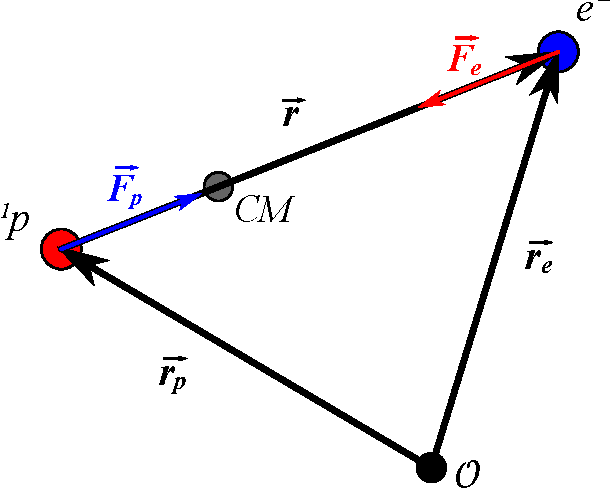
\includegraphics[width=.6\textwidth]{Analytisk-Mekanik/Brint.pdf}
% 	\caption{Illustration af brintatomet med arbitrært origo, $\mathcal{O}$, og massemidtpunkt $CM$. Derudover er kraften fra protonen på elektronen, $\va{F}_e$, indtegnet og farvet rød for at gøre den tydeligere, og ligeså for den blå kraft fra elektronen på protonen.}
% 	\label{mek:fig:Brint}
% \end{figure}
% %
% %
% \begin{opgave}{Brint}{2}
% \opg Eftersom $m_p\approx2000m_e$ er massemidtpunktet forskudt mod protonen således at at $\va{r}_e$ er i størrelsesordenen $2000\va{r}_p$. For at gøre tegningen overskuelig er massemidtpunktet angivet markant tættere på midten, se \cref{mek:fig:Brint}.
% \opg Afstanden mellem protonen og elektronen.
% \opg Se \cref{mek:fig:Brint}.
% \opg I massemidtpunktet, da problemet så reducerer til to generaliserede koordinater, idet der altid eksisterer en linje, som både protonen, elektronen og deres fælles massemidtpunkt befinder sig på.
% \opg Antagelsen giver mulighed for at benytte følgende approksimationer
% \begin{align*}
% 	&a) \quad m_p + m_e \simeq m_p, \\
% 	&b) \quad \frac{m_e}{m_p} \simeq 0,
% \end{align*}
% hvorved
% \begin{align*}
% 	\va{r}_\textsc{cm} &= \frac{m_e\va{r}_e + m_p\va{r}_p}{m_e + m_p} \\
% 	&\simeq \frac{m_e\va{r}_e + m_p\va{r}_p}{m_p} \\
% 	&= \frac{m_e}{m_p}\va{r}_e + \va{r}_p \\
% 	&\simeq \va{r}_p.
% \end{align*}
% \opg $\va{F} = -\dfrac{e^2}{4\pi\epsilon_0}\dfrac{\va{r}_e}{r_e^3}$ idet $\va{r}_p = 0$ i dette koordinatsystem.
% \end{opgave}


% \section*{Energi}
%
%
% \begin{opgave}{Energibevarelse}{1}
% \opg Det kunne være nogle af følgende: \\
% -- \: Kinetisk energi \\
% -- \: Potentiel energi \\
% -- \: Mekanisk energi \\
% -- \: Termisk energi \\
% -- \: Elektrisk energi \\
% -- \: Kemisk energi \\
% -- \: Bindingsenergi \\
% -- \: Masse \\
% -- \: Et cetera
% \opg Der er flere mulige forklaringer, men her er nogle forslag: \\
% -- \: En konservativ kraft er en kraft for hvilken arbejdet, den udfører, på et legeme under bevægelse fra et punkt til et andet, er uafhængig af vejen mellem de to punkter. \\
% -- \: En konservativ kraft er en kraft, der omsætter potentiel energi til kinetisk energi eller omvendt uden tab. \\
% -- \: En konservativ kraft er en kraft, der bevarer mekanisk energi. \\
% -- \: Hvis et legeme bevæger sig i en lukket bane og det totale arbejde fra en kraft et nul, da siges kraften at være konservativ.\\ 
% -- \: $\va{F}$ er konservativ, hvis
% \begin{align*}
% 	\oint\va{F}\cdot\d\va{l} = 0
% \end{align*}
% -- \: En konservativ kraft er udelukkende stedafhængig, og ethvert punkt i rummet kan derfor tildeles en potentiel energi.
% \opg Der er flere muligheder her. Til bevaret mekanisk energi kan det eksempelvis være: \\
% -- \: Bold i tyngdefelt i vakuum. \\
% -- \: Lod på fjeder, uden gnidning, små udsving. \\
% -- \: To ladede partikler. \\ \\
% Tre situationer, hvor mekanisk energi ikke er bevaret, kan eksempelvis være: \\
% -- \: Kugle skudt afsted under vand. \\
% -- \: Deformation af fjeder/andet materiale, over elastisk grænse. \\
% -- \: Uelastiske stød.
% \opg I de tre foreslåede eksempler: \\
% -- \: Kuglen påvirkes af vandmodstand. \\
% -- \: Der går energi til deformation af fjederen. \\
% -- \: Der går energi til deformation/sammensætning af de stødende legemer.
% \end{opgave}


% \begin{figure}
% 	\centering
% 	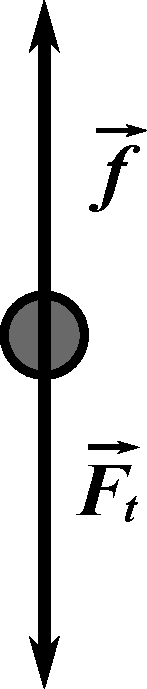
\includegraphics[width=.08\textwidth]{Analytisk-Mekanik/FritFald.pdf}
% 	\caption{Legemet er påvirket at en tyngdekraft $\va{F}_t$ og en friktionskraft $\va{f}$.}
% 	\label{mek:fig:FritFald}
% \end{figure}
% %
% %
% \begin{opgave}{Frit fald}{1}
% \opg Se \cref{mek:fig:FritFald}.
% \opg Friktion er ikke en konservativ kraft, idet den omsætter kinetisk energi til termisk energi i stedet for potentiel energi.
% \opg Negliceres friktion er der energibevarelse, hvorfor
% \begin{align*}
% 	\frac{1}{2}mv_0^2 + mgh &= \frac{1}{2}mv^2 + mg(0) \\
% 	\xRightarrow{v_0=0} mgh = \frac{1}{2}mv^2 \\
% 	v = \sqrt{2gh}
% \end{align*}
% \opg Hvis $h$ er meget stor er den en dårlig antagelse, idet legemet vil nå sin terminalhastighed, før den rammer Jorden. Negligeres friktionen ophører terminalhastigheden med at eksistere, hvilket gør antagelsen dårlig. \\
% Luftmodstand beskrives ofte på en af de to følgende former:
% \begin{align*}
% 	\va{f} =
% 		\begin{cases}
% 			-c_1v \\
% 			-c_2v^2
% 		\end{cases}
% \end{align*}
% hvor $v$ er hastigheden og $c_i$ er konstanter, som afhænger af legemets udformning. For at friktionskraften skal være negligibel, må konstanterne $c_i$ være relativt små, og $h$ skal være tilpas lille til at hastigheden ikke når at blive for stor, hvorfor et bud på et sæt af kriterier er
% \begin{align*}
% 	h &\ll 2g,\\
% 	c_i &< 1.
% \end{align*}
% Der er ikke noget entydigt rigtigt svar, da problemet ikke skal analyseres grundigt nok til at gøre dette stringent, men der bør fremgå en fysisk forståelse for situationen af kriteriet.
% \end{opgave}


% \begin{opgave}{Kollisioner}{1}
% \opg Newtons 3. lov.
% \opg Newtons 3. lov giver at kraften er lige stor og modsatrettet.
% \opg Af det ovenstående er
% \begin{align*}
% 	\va{F}_1 = -\va{F}_2,
% \end{align*}
% hvorved Newtons 2. lov siger at den samlede kraft på systemet er
% \begin{align*}
% 	\va{F}_1 + \va{F}_2 &= \dif{t}{}(\va{p}_1 + \va{p}_2) \\
% 	\va{F}_1 - \va{F}_1 &= \dif{t}{}(\va{p}_1 + \va{p}_2) \\
% 	0 &= \dif{t}{}(\va{p}_1 + \va{p}_2).
% \end{align*}
% Ergo er den totale impuls bevaret.
% \opg Af \cref{mek:opg:Energibevarelse} er et legemes mekaniske energi bevaret, hvis legemet kun er påvirket af konservative kræfter. Da der er set bort fra eventuelle ydre kræfter, er den potentielle energi i systemet $V=0$, hvorfor den kinetiske energi er bevaret, hvis legemerne kun påvirker hinanden med konservative kræfter. \\
% a) Af definitionen af et elastisk stød, er legemerne kun påvirket af konservative kræfter, hvorfor den kinetiske energi er bevaret. \\
% b) Uelastiske kollisioner er alle kollisioner, hvor legemerne påvirker hinanden på en måde, der er ikke er konservativ, hvorfor den kinetiske energi ikke er bevaret.
% \end{opgave}

\section*{Approksimation til harmonisk oscillator}
\begin{opgave}[2]{Bevægelse omkring ligevægt}
%
\opg $\dv*{V}{r} = V_0\left(\frac{1}{R} - \lambda^2\frac{R}{r^2}\right)$
%
\opg Ligevægtspunktet bestemmes ved at sætte den afledede til nul og benytte nulreglen:
%
\begin{align*}
	0 &= \dv*{V}{r}, \\
	\implies \frac{1}{R} &= \lambda^2\frac{R}{r^2}, \\
	\implies r_0 &= \lambda R.
\end{align*}
%
\opg Den andenafledte er:
%
\begin{align*}
	\dv[2]{V}{r} = \frac{2V_0R\lambda^2}{r^3}.
\end{align*}
%
\opg Der er tale om et minimum, hvis den anden afledede evalueret i minimaet er positiv. Det gælder da alle konstanterne er antaget positive.
%
\begin{align*}
	\left.\dv[2]{V}{r}\right|_{r = \lambda R} = \left.\frac{2V_0R\lambda^2}{r^3}\right|_{r = \lambda R} = \frac{2V_0}{\lambda R^2} > 0.
\end{align*}
%
\opg Først isoleres $r$ i definitionen af $x$ og derefter indsættes det i funktionen $V(r)$.
%
\begin{align*}
	r &= x + r_0 \\
	\implies V(x) &= V_0\left(\frac{x + r_0}{R} + \lambda^2\frac{R}{x + r_0}\right)
\end{align*}
%
\opg Taylorudviklingen af en funktion $f(x)$ omkring $x=0$ til anden orden er
%
\begin{align*}
	f(x) \simeq f(0) + x\left.\dv{f(x)}{x}\right|_{x=0} + x^2\left.\frac{1}{2}\dv[2]{f(x)}{x}\right|_{x=0}.
\end{align*}
%
I første omgang bestemmes potentialets minimum
%
\begin{align*}
	V(x=0) &= V_0\left(\frac{\lambda R}{R} + \lambda^2\frac{R}{\lambda R}\right) \\
	&= 2V_0\lambda.
\end{align*}
%
Herefter bestemmes den første afledede evaluerede i nul
%
\begin{align*}
	 \left.\dv{f(x)}{x}\right|_{x=0} &= \left[\frac{V_0}{R} - V_0\lambda^2\frac{R}{(x+r_0)^2}\right]_{x=0} \\
	 &= \frac{V_0}{R} - V_0\lambda^2\frac{R}{r_0^2} \\
	 &= \frac{V_0}{R} - V_0\lambda^2\frac{R}{(\lambda R)^2} \\
	 &= \frac{V_0}{R} - \frac{V_0}{R} = 0.
\end{align*}
%
Så den anden afledede
%
\begin{align*}
	 \left.\dv[2]{f(x)}{x}\right|_{x=0} &= \left[\dv{f(x)}{x}\left(\frac{V_0}{R} - V_0\lambda^2\frac{R}{(x+r_0)^2}\right)\right]_{x=0} \\
	 &= \left.\frac{2V_0R\lambda^2}{(x+r_0)^3}\right|_{x=0} \\
	 &= \frac{2V_0Rr_0\lambda^2}{r_0^3} \\
	 &= \frac{2V_0R\lambda^2}{(R\lambda)^3} \\
	 &= \frac{2V_0}{\lambda R^2}.
\end{align*}
%
Dermed bliver den potentielle energi omkring ligevægtspunktet $r_0$
%
\begin{align*}
	V(x) \simeq 2V_0\lambda + \frac{1}{2}\frac{2V_0}{\lambda R^2}x^2 = c + \frac{1}{2}kx^2,
\end{align*}
%
hvor $c$ og $k$ er defineret som
%
\begin{align*}
	c &= 2V_0\lambda,\\
	k &= \frac{2V_0}{\lambda R^2}.
\end{align*}
%
Supplerende kan de siges at nulpunktet for potentiel energi er arbitrært, hvorfor $V = (1/2)kx^2$ er lige så validt et potential at benytte.
%
\opg Vinkelfrekvensen for den harmoniske oscillator er
%
\begin{align*}
	\omega = \sqrt{\frac{k}{m}} = \left(\frac{2V_0}{m\lambda R^2}\right)^{1/2}.
\end{align*}
%
Er det ikke oplagt at vinkelfrekvensen for en harmonisk oscillator opfylder at $\omega^2 = k/m$, så kan der henvises til de forskellige beskrivelser af pendulet, det vil sige \cref{k-mek:ex:pendul_newton,k-mek:ex:PendulLagrange} i kompendiet.
\end{opgave}


\begin{opgave}[2]{(Næsten) alt er en harmonisk oscillator}
%
\opg Potentialet er arbitrært, så det indsættes bare i \cref{k-mat:eq:Taylor_pol} i kompendiet analogt til eksemplet med $e^x$
%
\begin{align} \label{mek:eq:VTaylor}
	V(x) \simeq V(x=0) &+ x\left.\dv{V(x)}{x}\right|_{x=0} + \frac{1}{2}x^2\left.\dv[2]{V(x)}{x}\right|_{x=0}.
\end{align}
%
Der kan ikke gøres mere, da $V(x)$ er ukendt.
\opg Sammenlignes \cref{mek:eq:VTaylor} med med den harmoniske oscillator, $f(x)$, i opgaven, ses det at
%
\begin{align*}
	c &= V(x=0), \\
	k &= \left.\dv[2]{V(x)}{x}\right|_{x=0},
\end{align*}
%
idet de afledede bliver en konstant, når de evalueres i et punkt. Ledet $x\left.\dv{V(x)}{x}\right|_{x=0}$ passer dog ikke ind, og kriteriet må derfor være at dette er nul for alle værdier af $x$, hvorfor differentialet må være nul:
%
\begin{align*}
	\left.\dv{V(x)}{x}\right|_{x=0} = 0 \enspace\forall \; x \implies \dv{V(x)}{x} = 0.
\end{align*}
%
\opg Det kunne være følgende funktioner, hvor store bogstaver er konstanter
%
\begingroup
\allowdisplaybreaks
%
\begin{align*}
	\text{Parabel uden førstegradsled:} \qquad
	&f(x) = A + Bx^2 \\
	\text{Gaussfunktion:} \qquad
	&f(x) = -Ae^{-Bx^2}\\
	\text{Cirkel:} \qquad
	&f(x) = \frac{\pm A}{\sqrt{1-x^2}}\\
	\text{Morsepotentiale:} \qquad
	&f(x) = A\left(1-e^{-Bx}\right)^2\\
	\text{Potentialet fra \cref{mek:opg:equilibrium}:} \qquad
	&f(x) = A\left(\frac{x}{B}+C^2\frac{B}{x}\right)\\
	\text{Effektivt potentiale for planetbevægelse:} \qquad
	&f(x) = \frac{A}{x^2}-\frac{B}{x} \\
	\text{Trigonometrisk:} \qquad
	&f(x) = A\cos(Bx + C) + D \\
	\text{Hyperbolsk cosinus:} \qquad
	&f(x) = A\left(e^{(Bx)} + e^{(-Bx)}\right) = 2A\cosh(Bx) \\
	\text{Og så videre:} \qquad &f(x) = ... 
\end{align*}
%
\endgroup
%
Cosinus og den hyperbolske cosinus kræver dog at de evalueres i et punkt, hvor henholdsvis sinus og sinus hyperbolsk er nul. Dermed kan sinus (hyperbolsk) også bruges under samme betingelser.
\opg $V(x)$ og $\tilde{V}(x)$ opfører sig ens hvis deres afledede er ens
%
\begin{align*}
	\pdv{\tilde{V}(x)}{x} = \pdv{V(x)}{x} + \pdv{\lambda} \xleq{\partial\lambda/\partial x = 0} \pdv{V(x)}{x},
\end{align*}
%
da $\lambda$ er en konstant.
%
\opg Eftersom $c$ er en konstant gælder det samme for den, som for $\lambda$, hvorfor den kan lægges til med modsat fortegn. Derfor vælges $\lambda = -c$, hvorved den harmoniske oscillators potentielle energi kan skrives som
%
\begin{align*}
	\tilde{V}(x) = V(x) - c = \frac{1}{2}kx^2.
\end{align*}
%
\end{opgave}


\section*{Etlegemeproblemer}


\begin{opgave}[1]{Klods på en fjeder}
%
Lagrangeformalismen bygger på systemets energier, hvorfor disse bestemmes først.
%
\opg Den kinetiske energi er
%
\begin{align*}
	K &= \frac{1}{2}m\dot{x}^2
\end{align*}
%
\opg Den potentielle energi er
%
\begin{align*}
	K &= \frac{1}{2}m\dot{x}^2
\end{align*}
%
\opg Dermed bliver Lagrangefunktionen
%
\begin{align*}
	L = K - V = \frac{1}{2}m\dot{x}^2 - \frac{1}{2}kx^2.
\end{align*}
%
\opg For at indsætte i Euler-Lagrangeligningen skal nogle differentialer bestemmes
%
\begin{align*}
	\dv{L}{x} &= -kx,\\
	\dv{L}{\dot{x}}&= m\dot{x}, \\
	\el{x} &= m\ddot{x}.
\end{align*}
%
Dette indsættes i Euler-Lagrangeligningen
%
\begin{align*}
	m\ddot{x} = -kx,
\end{align*}
%
hvilket er magen til \cref{k-mek:eq:FjederDiffLign} i kompendiet.
\end{opgave}


\begin{opgave}[1]{Atwoods faldmaskine}
%
\opg Snorlængden er konstant, og af tegningen, \cref{mek:fig:Atwood}, fremgår det at længden af snoren kan udtrykkes som
%
\begin{align*}
	l = x + y + \pi R.
\end{align*}
%
Da $R$ og $l$ er konstanter kan $y$ udtrykkes ved $x$ som
%
\begin{align} \label{mek:eq:xAtwood}
	y = l - x - \pi R.
\end{align}
%
\opg Differentieres \cref{mek:eq:xAtwood} med hensyn til tid fås
%
\begin{align} \label{mek:eq:AtwoodFart}
	\dot{y} = -\dot{x},
\end{align}
%
idet $l,\pi,R$ er konstanter.
%
\opg Den potentielle energi findes ved at bruge formlen $V = mgh$ hvor $h$ er forskydningen fra nulpunktet. Hvert lod er forskudt henholdsvis $x$ og $y$ i negativ retning, hvorfor
%
\begin{align} \label{mek:eq:VAtwood}
	V = -g(m_1x + m_2y).
\end{align}
%
Dette skyldes at nulpunktet for den potentielle energi for hvert lod er valgt til henholdsvis $x=0$ og $y=0$. Den potentielle energi skal så falde, når for hvert lod skal så falde, når henholdsvis $x$ og $y$ bliver mindre, hvilket giver fortegnet i \cref{mek:eq:VAtwood}. \\
Er man stor modstander af konceptet om negativ potentiel energi, så kan man definere nulpunktet i afstanden $H$ under faldmaskinen. Derved bliver den højde, $h$, der er relevant for den potentielle energi, henholdsvis
%
\begin{align*}
	h_1 = H - x
\end{align*}
%
og
%
\begin{align*}
	h_2 = H - y,
\end{align*}
%
hvor subscribtet angiver hvilket lod, der er tale om.
%
\opg For kinetisk energi kastes ind i formlen $K = \sum_i\frac{1}{2}m_iv_i^2$, så der fås
%
\begin{align*}
	K = \frac{1}{2}(m_1\dot{x}^2 + m_2\dot{y}^2) =.
\end{align*}
%
\opg Lagrangefunktionen er pr. definition $L = K - V$. Bruges dette samt ligninger
\cref{mek:eq:xAtwood} og \cref{mek:eq:AtwoodFart} fås
%
\begin{align*}
	L &= K - V \\
	&= \frac{1}{2}(m_1\dot{x}^2 + m_2\dot{y}) - (-g)(m_1x + m_2y) \\
	&=  \frac{1}{2}(m_1\dot{x}^2 + m_2(-\dot{x})^2) + g\Big[m_1x + m_2(l - x - \pi R)\Big] \\
	&= \frac{1}{2}(m_1+m_2)\dot{x}^2 + g\Big[m_1x + m_2(l - x - \pi R)\Big].
\end{align*}
%
Havde man placeret nulpunktet for den potentielle energi afstanden $H$ under faldmaskinen, ville Lagrangefunktionen blive
%
\begin{align*}
	L = \frac{1}{2}(m_1+m_2)\dot{x}^2 - g\Big[m_1(H-x) + m_2(H - l + x + \pi R)\Big].
\end{align*}
%
Den eneste forskel på de to Lagrangefunktioner er konstanter, og de forsvinder alligevel ved differentiation. Dette bruger konceptet at enhver Langrangefunktion, der giver den rigtige bevægelse, er en gyldig Lagrangefunktion, hvilket \cref{mek:opg:HO} også illustrerer.
%
\opg For at benytter Euler-Lagrangeligninger skal følgende differentialer bruges
%
\begin{align} \label{mek:eq:AtwoodEL}
	\pdv{L}{x} &= g(m_1 - m_2) \\
	\pdv{L}{\dot{x}} &= (m_1 + m_2)\dot{x} \\
	\el{x} &= (m_1 + m_2)\ddot{x}
\end{align}
%
Bruges Euler-Lagrangeligningen, \cref{k-mek:eq:Euler-Lagrange} i kompendiet, til at sætte første og sidste udtryk i \cref{mek:eq:AtwoodEL} fås
%
\begin{align*}
	(m_1 + m_2)\ddot{x} &= g(m_1 - m_2) \\
	\ddot{x} &= g\frac{m_1 - m_2}{m_1 + m_2}
\end{align*}
%
\opg Både $g$ og $m_1+m_2$ er positive led, hvorfor fortegnet er bestemt af tælleren.
%
\begin{align*}
	m_1>m_2: \quad m_1-m_2>0 \implies \ddot{x}>0 \\
	m_2>m_1: \quad m_1-m_2<0 \implies \ddot{x}<0
\end{align*}
%
Dette stemmer overens med det forventede, idet $\ddot{x}>0$ betyder at accelereres i positiv $x$-retningen, hvilket betyder at $m_1$ falder ned, mens $m_2$ trækkes op. Dette sker lige netop når $m_1>m_2$, hvilket også giver fysisk mening, idet det tungeste lod burde falde ned, og trække det letteste med sig. Der gælder det omvendte, hvis $m_2>m_1$.
%
\opg Udføres integralet fås
%
\begin{align*}
	x(t) &= \iint a \dd{t} \dd{t} \\
	&= \int at + v_0 \dd{t} \\
	&= \frac{1}{2}at^2 + v_0t + x_0 \\
	&= \frac{1}{2}g\frac{m_1 - m_2}{m_1 + m_2}t^2 + v_0t + x_0.
\end{align*}
%
\end{opgave}


\begin{opgave}[2]{Partikel på en cylinder}
%
\opg Siden partiklen er fastlåst på overfladen af cylinderen er $r$ koordinatet altid lig radien af cylinderen:
%
\begin{align}
	r = R.
\end{align}
%
Resten er frie.
%
\opg Lad os starte med den letteste: $z$. Der er det samme i kartesiske og cylindriske koordinater.
%
\begin{align}
	\dot{z} = \dot{z}.
\end{align}
%
De to andre afhænger kun af $\phi$, så efter kædereglen følger:
%
\begin{align*}
	\dot{x} &= -R\dot{\phi} \sin(\phi)\\
	\dot{y} &= R\dot{\phi} \cos(\phi)
\end{align*}
%
\opg I kartesiske koordinater er:
%
\begin{align}
    v^2 = \dot{x}^2 + \dot{y}^2 + \dot{z}^2
\end{align}
%
Vi kan her bruge Pythagoras sætning for enhedstrekanten:
%
\begin{align}
	\cos^2(\phi)+\sin^2(\phi) = 1
\end{align}
%
Så den kinetiske energi er:
%
\begin{align*}
	K &= \frac{1}{2}mv^2 \\
	&= \frac{m}{2}(R^2\dot{\phi}^2\sin^2(\phi)+R^2\dot{\phi}^2\cos^2(\phi)+\dot{z}^2)\\
	&= \frac{m}{2}(R^2\dot{\phi}^2+\dot{z}^2).
\end{align*}
%
\opg Siden potentialet er nul er Lagrangefunktionen:
%
\begin{align}
	L = K = \frac{m}{2}(R^2\dot{\phi}^2+\dot{z}^2).
\end{align}
%
\opg Generelt er en Euler-Lagrangeligning på formen:
%
\begin{align}
	\el{q} = \pdv{L}{q}
\end{align}
%
Igen lad os starte med $z$.
%
\begin{align*}
	\pdv{L}{\dot{z}} &= m\dot{z}\\
	\el{z} &= m\ddot{z}\\
	\pdv{L}{L} &= 0
\end{align*}
%
Det giver Euler-Lagrangeligningen for $z$:
%
\begin{align}
	m\ddot{z} = 0
\end{align}
%
Tilsvarende for $\phi$
%
\begin{align*}
	\pdv{L}{\dot{\phi}} &= mR^2\dot{\phi}\\
	\el{\phi} &= mR^2\ddot{\phi}\\
	\pdv{L}{\phi} &= 0
\end{align*}
%
Det giver Euler-Lagrangeligningen for $\phi$:
%
\begin{align}
	mR^2\ddot{\phi} = 0
\end{align}
%
Begge differentialligninger kan reduceres så vi ender med:
%
\begin{align*}
	\ddot{z} &= 0,\\
	\ddot{\phi} &= 0.
\end{align*}
%
\opg Begge differentialligninger giver bevægelse med konstant hastighed. For $z$ er det konstant hastighed langs cylinderaksen. For $\phi$ er det cirkulær bevægelse omkring aksen. Kombineret giver det en spiralbevægelse. Som en bonus er løsningen til bevægelsesligningerne:
%
\begin{align*}
	z(t) &= v_z t+z_+0 \\
	\phi(t) &= \omega t + \phi_0 \\
	x(t) &= R\cos(\omega t+\phi_0) \\
	y(t) &= R\sin(\omega t + \phi_0)
\end{align*}
%
\end{opgave}


\begin{opgave}[2]{Yoyo}
%
% De ligninger, der henvises til siger at
% %
% \begin{align*}
% 	K &= \frac{1}{2}mv_\textsc{cm}^2 + \frac{1}{2}I\omega^2, \\
% 	v &= r\dot{\phi} = r\omega.
% \end{align*}
% %
% \opg Fra opgaven er $v = v_\textsc{cm} = \dot{z}$  da yoyoen kun bevæger sig translatorisk i $z$-retningen. Kombineres alt dette med informationen om intertimomentet fås
% %
% \begin{align*}
% 	K &\xleq{v=r\omega} \frac{1}{2}mv_\textsc{cm}^2 + \frac{1}{2}I\left(\frac{v}{r}\right)^2 \\
% 	&\xleq{v=v_\textsc{cm}=\dot{z}} \frac{1}{2}m\dot{z}^2 + \frac{1}{2}I\left(\frac{\dot{z}}{r}\right)^2 \\
% 	&\xleq{I = \frac{1}{2}mR^2} \frac{1}{2}m\dot{z}^2 + \frac{1}{4}mR^2\left(\frac{\dot{z}}{r}\right)^2.
% \end{align*}
%
\opg Den potentielle gravitationelle energi er $V = mgh$, hvor $h$ er den afstanden til nulpunktet i tyngdekraftens retning. Defineres nulpunktet sådan at $V(z=0)=0$ er $z=-h$, fordi $V$ skal blive mindre, når $z$ bliver større, hvorved $V = -mgz$. Her kan igen gøres det samme med at definere $V(x) = 0$ til et sted langt nede, og dermed indføre en konstant i den potentielle energi, som senere forsvinder ved differentiation.
%
\opg Benyttes definitionen af Lagrangefunktionen inden der sættes udenfor parentes fås
%
\begin{align*}
	L &= K - V \\
	&= \frac{1}{2}m\dot{z}^2 + \frac{1}{4}mR^2\left(\frac{\dot{z}}{r}\right)^2 - (-mgz) \\
	&= \frac{1}{2}m\left[1 + \frac{1}{2}\left(\frac{R}{r}\right)^2\right]\dot{z}^2 + mgz.
\end{align*}
%
\opg De afledede af Lagrangefunktionen er
%
\begin{align*}
	\pdv{L}{z} &= mg,\\
	\pdv{L}{L}{\dot{z}} &= m\left[1 + \frac{1}{2}\left(\frac{R}{r}\right)^2\right]\dot{z}, \\
	\el{z} &= m\left[1 + \frac{1}{2}\left(\frac{R}{r}\right)^2\right]\ddot{z}.
\end{align*}
%
\opg Euler-Lagrangeligningen siger at det første og sidste differentiale er lig hinanden\footnote{Lighedstegnet vendes om tilsidst, da det ser pænest ud.}
%
\begin{align*}
	\pdv{L}{z} &= \el{z}\\
	mg &= m\left[1 + \frac{1}{2}\left(\frac{R}{r}\right)^2\right]\ddot{z} \\
	g &= \left[1 + \frac{1}{2}\left(\frac{R}{r}\right)^2\right]\ddot{z} \\
	\ddot{z} &= \frac{g}{1 + \frac{1}{2}\left(\frac{R}{r}\right)^2}.
\end{align*}
%
\opg Yoyoen er beskrevet af samme bevægelsesligning, som den for frit fald fra kompendiet, \cref{k-mat:eq:position}. Frit fald er bevægelse med konstant acceleration, hvilket også er tilfældet for yoyoen. Accelerationen er dog ikke tyngdeaccelerationen, men $g/(1 + (R/r)^2/2)$. Yoyoen accelereres derfor langsommere end tilfældet er for almindeligt frit fald. Dette skyldes at yoyoen drejer rundt, hvorfor den potentielle energi omdannes både til translatorisk og rotationel, kinetisk energi. Det bremser derfor yoyoen, at den drejer rundt.
%
\opg Med Newtonsk mekanik ville man være nød til at bestemme summen af kræfter og summen af kraftmomenter, der begge vil afhænge af snorkraften i snoren, $S$. Denne er ukendt, og derfor besværlig at regne med. Derudover ville man skulle bruge både Newtons 2. lov og Newtons 2. lov for roterende bevægelse, og så kæde det sammen gennem den ukendte snorkraft, hvilket er ret så omstændigt, sammenlignet med hvor elegant det er at benytte Lagrangemekanikken.
\end{opgave}

\begin{opgave}[3]{Elektriske kredsløb og kvantecomputere}
%
\opg For at benytte Euler-Lagrangeligning skal de nødvendige differentialer bestemmes:
%
\begin{align*}
    \pdv{L}{\phi} &= -E_\textup{J}\sin(\phi), \\
    \pdv{L}{\dot{\phi}} &= C\dot{\phi}, \\
    \el{\phi} &= C\ddot{\phi}.
\end{align*}
%
Indsættes dette i Euler-Lagrangeligningen fås
%
\begin{align} \label{mek:eq:transmon_eom_facit}
    \ddot{\phi} = - \frac{E_\textup{J}}{C}\sin(\phi),
\end{align}
%
som ønsket vist.
\opg Fra \cref{mek:eq:transmon_eom_facit} ses at $\omega = \sqrt{E_\textup{J}/C}$.
%
\opg Pendulet; se \cref{k-mek:ex:PendulLagrange} i kompendiet.
%
\opg For små vinkler kan sinus approksimeres med ledene til og med første orden i dens Taylorrække, hvorfor $\sin(\phi) \simeq \phi$. Derved fås
%
\begin{align*}
    \ddot{\phi} \simeq - \frac{E_\textup{J}}{C} \phi.
\end{align*}
%
\opg Det gælder for små vinkler. Mere specifikt skal tredjeordensledet (andenordensledet er 0) være meget mindre end førsteordensledet
%
\begin{align} \label{mek:eq:sinus_1.orden}
    \frac{\phi^3}{3!} \ll \phi \iff \phi \ll \sqrt{3!} = \sqrt{6}.
\end{align}
%
\opg Taylorrækken for sinus til 3. orden er
%
\begin{align*}
    \sin(\phi) \simeq \phi + \frac{1}{3!}\phi^3.
\end{align*}
%
Derfor er \cref{mek:eq:transmon_eom_facit} til fjerde orden
%
\begin{align}
    \ddot{\phi} \simeq - \frac{E_\textup{J}}{C} \phi + \frac{E_\textup{J}}{3!C} \phi^3.
\end{align}
%
Derved er $K_3 = E_\textup{J}/(3!C) = E_\textup{J}/(6C)$.
%
\opg Vinklerne skal igen være små, men de skal heller ikke hele tiden være så små, at \cref{mek:eq:sinus_1.orden} altid er opfyldt. Med andre ord skal vinklerne være små, men ikke for små. Hvad der altid skal være opfyldt er at femteordensledet er lille
%
\begin{align} \label{mek:eq:sinus_3.orden}
    \frac{\phi^5}{5!} \ll \frac{\phi^3}{3!} \iff \phi \ll \sqrt{\frac{5!}{3!}} = \sqrt{5\cdot4} = \sqrt{20}.
\end{align}
%
\end{opgave}

% \begin{figure}[t]
% \centering
% 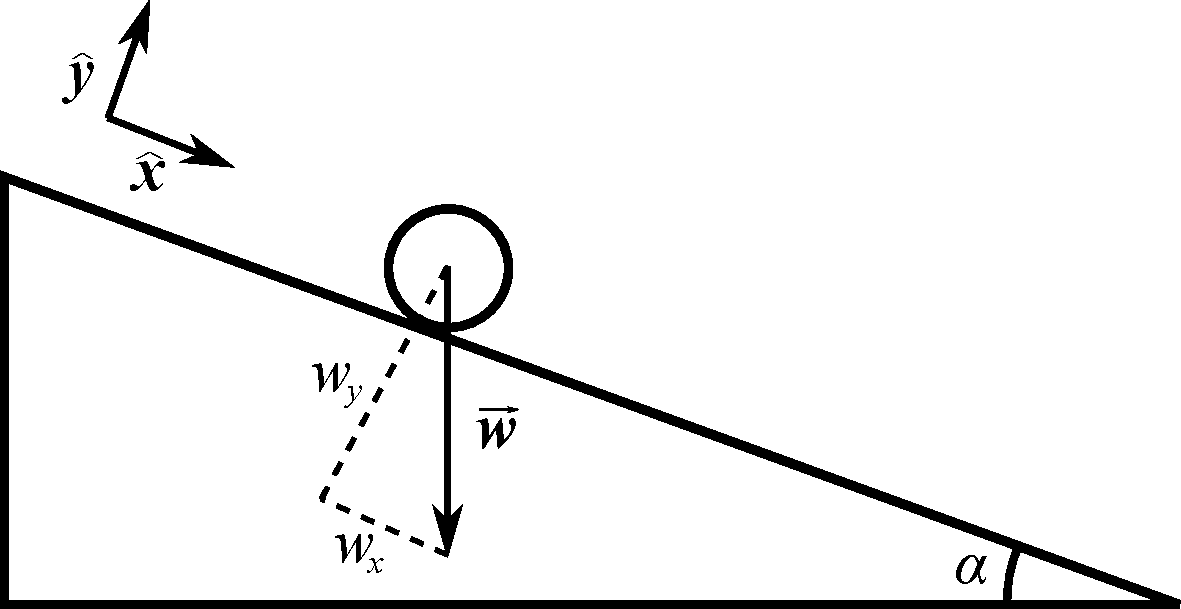
\includegraphics[width=.6\columnwidth]{Analytisk-Mekanik/Cylinder.pdf}
% \caption{Eksempel på bevarelse af spørgsmålene 1 og 2 i \cref{mek:opg:cylinder}. Vinklen $\alpha$ skal lokaliseres, $x$ skal defineres parallelt med skråplanet og identificeres som generaliseret koordinat.}
% \label{mek:fig:Cylinder}
% \end{figure}
% %
% %
% \begin{opgave}[2]{Cylinder på skråplan}
% %
% \opg Se \cref{mek:fig:Cylinder}.
% %
% \opg Fremgår ligeså af figuren.
% %
% \opg Den potentielle energi opskrives ud fra højden over bunden af skråplanet $h = x\sin(\alpha)$. Dermed bliver den potentielle energi
% %
% \begin{align*}
% 	V = mg\sin(\alpha)x.
% \end{align*}
% %
% \opg Den kinetiske energi er
% %
% \begin{align*}
% 	K &= \frac{1}{2}m\dot{x}^2 + \frac{1}{2}I\omega^2 \\
% 	&= \frac{1}{2}m\ddot{x}^2 + \frac{1}{2}I\left(\frac{\dot{x}}{^R}\right)^2 \\
% 	&= \frac{1}{2}\left(m+\frac{I}{R^2}\right)\dot{x}^2,
% \end{align*}
% analogt til spørgsmål 1 i \cref{mek:opg:Yoyo}.
% \opg Den potentielle energi er
% \begin{align*}
% 	L &= K + V = \frac{1}{2}\left(m+\frac{I}{R^2}\right)\dot{x}^2 - mg\sin(\alpha)x.
% \end{align*}
% \opg Der differentieres
% \begin{align*}
% 	\pdif{\dot{x}}{L} &= \left(m+\frac{I}{R^2}\right)\dot{x}, \\
% 	\pdif{x}{L} &= -mg\sin(\alpha)x, \\
% 	\implies \el{x} &= \left(m+\frac{I}{R^2}\right)\ddot{x}.
% \end{align*}
% Differentialerne løses i rækkefølge som
% \begin{align*}
% 	\pdif{x}{}\frac{1}{2}x^2 &= x,\\
% 	\pdif{x}{}x &= 1,\\
% 	\dif{t}{}\dot{x} &= \ddot{x}.
% \end{align*}
% Nu stoppes ind i Euler-Lagrangeligningen og divideres først med parentesen og til sidst forkortes brøken med $m$:
% \begin{align*}
% 	\el{x} &= \pdif{x}{L} \\
% 	\implies \ddot{x} &= -\frac{g\sin\alpha}{1+I/mR^2}.
% \end{align*}
% \opg Bevægelsesligningen afhænger ikke $t,x,\dot{x}$, hvorfor der ikke sker nogen ændring i accelerationen mens tiden går.
% \opg Bevægelsesligningen skrives på formen
% \begin{align*}
% 	\dif[2]{t}{x} &= \tilde{g} \\
% 	\implies x &= \int\int\tilde{g}\dd{t}^2 \\ 
% 	&= \integral{\tilde{g}t + v_0}{t}{}{} \\
% 	&= \frac{1}{2}\tilde{g}t^2 + v_0t + x_0 : .
% \end{align*}
% \end{opgave}


\begin{opgave}[3]{Masse på roterende ring}
%
Dette problem har mange paralleller til pendulet, hvorfor det kan være relevant at referere til \cref{k-mek:ex:PendulLagrange} i kompendiet.
%
\opg Gravitationel potentiel energi er på formen $V=mgh$, og helt ækvivalent til pendulet defineres nulpunktet i $\phi = 0$, hvorved
%
\begin{align*}
	V(\phi) = mgR\big[1 - \cos(\phi)\big].
\end{align*}
%
\opg \cref{k-mek:eq:SmartFart} i kompendiet siger at $v = r\dot{\phi}$, men den skal lige vendes rigtigt, for at kunne bruges her. Den er udledt for cylinderkoordinater, men gælder generelt for cirkelbevægelser, hvorfor de rigtige cirkler skal identificeres. Hastigheden for lodets bevægelse langs ringen, har radius bliver $R$ og vinkelhastighed $\dot{\phi}$, hvorfor
%
\begin{align*}
	v_\textup{lod} = R\dot{\phi}.
\end{align*}
%
Den anden cirkel kræver lidt mere at forestille sig. Forestiller man sig at massen fastholdes samme sted på ringen, vil den være i jævn cirkelbevægelsen i planet ortogonalt på tegningen. Denne cirkelbevægelse har vinkelhastighed $\omega$ og radius $\rho$, og trigonometri kan bruges til at udtrykke $\rho$ ved $\phi$.
%
\begin{align*}
	v_\textup{ring} = \rho\omega \xleq{\rho = R\sin(\phi)} R\omega\sin(\phi).
\end{align*} 
%
\opg Den totale kvadrerede hastighed bliver nu summen af kvardraterne på komponenterne
%
\begin{align*}
	v^2 &= v_\textup{lod}^2 + v_\textup{ring}^2 \\
	&= R^2\dot{\phi}^2 + R^2\omega^2\sin^2(\phi) \\
	&= R^2\big[\dot{\phi}^2 + \omega^2\sin^2(\phi)\big].
\end{align*}
%
Ganges dette med $m/2$ fås den kinetiske energi
%
\begin{align*}
	K = \frac{1}{2}mR^2\big[\dot{\phi}^2 + \omega^2\sin^2(\phi)\big].
\end{align*}
%
og trækkes den potentielle energi fra fås
%
\begin{align*}
	L = \frac{1}{2}mR^2\big[\dot{\phi}^2 + \omega^2\sin^2(\phi)\big] - mgR\big[1-\cos(\phi)\big].
\end{align*}
%
\opg For at benytte Euler-Lagrangeligningen til at bestemme bevægelsesligningen bestemmes følgende differentialer
%
\begin{align*}
	\pdv{L}{\dot{\phi}} &= mR^2\dot{\phi}, \\
	\el{\phi} &= mR^2\ddot{\phi}, \\
	\pdv{L}{\phi} &= mR^2\omega^2\sin(\phi)\cos(\phi) - mgR\sin(\phi).
\end{align*}
%
hvor kædereglen skal huskes til differentiation af $\sin^2(\phi)$ i det sidste differential. Euler-Lagrangeligningen siger så at de to sidste differentialer er ens, hvorfor
%
\begin{align} \label{mek:eq:BeadOnHoopEOM}
	\begin{aligned}
		\el{\phi} &= \pdv{L}{\phi} \\
		mR^2\ddot{\phi} &= mR^2\omega^2\sin(\phi)\cos(\phi) - mgR\sin(\phi) \\
		\ddot{\phi} &= \left[\omega^2\cos(\phi) - \frac{g}{R}\right]\sin(\phi).
    \end{aligned}
\end{align}
%
\opg Fysisk set er et ligevægtspunkt et sted, hvor et objekt bliver, hvis det placeres der med farten $0$. Stabiliteten kan undersøges ved at placere objektet der med hastigheden nul, og så puffe en smule til det. Accelereres objektet tilbage mod ligevægtspunktet, er ligevægtspunktet stabilt, men accelereres det væk fra er det ustabilt. Som eksempel kan tænkes på en bold i et bakket område. Placeres bolden præcis på toppen af en bakke, så bliver den der, men skubbes der en smule til den, triller den ned af bakken. Derfor er bakketoppen et ustabilt ligevægtspunkt. Placeres bolden dog midt i en bakkedal uden fart, bliver bolden der også, men puffes der til den, vil den rulle lidt op ad bakken inden den ruller ned igen og tilbage til ligevægtspunktet. Derfor er dette punkt stabilt. \\
Kaldes et ligevægtspunkt $\phi_0$, så kan disse kriterier udtrykkes matematisk ved at $\ddot{\phi}|_{\phi=\phi_0} = 0$, hvis $\dot{\phi}|_{\phi=\phi_0} = 0$ og $\phi = \phi_0$. For at undersøge stabiliteten lader man $\phi$ være forskudt både lidt i positiv og i negativ, og hvis $\ddot{\phi}$ så også er har modsat fortegn af forskydningen, er ligevægtspunktet stabilt. Hvis ikke er ligevægtspunktet ustabilt.
%
\opg Af ovenstående sættes $\ddot{\phi} = 0$
%
\begin{align*}
	0 = \ddot{\phi} &= \left[\omega^2\cos(\phi) - \frac{g}{R}\right]\sin(\phi) \\
	\implies 0 &= \begin{cases} \omega^2\cos(\phi_0) - \dfrac{g}{R} \\[1mm]
	\sin(\phi_0) \end{cases} \\
	%
	\implies \phi_0 &= \begin{cases}
	\textup{Re}\left[\pm\cos^{-1}\left(\dfrac{g}{R\omega^2}\right)\right] \\[1mm]
	\sin^{-1}(0) = 0,\pm\pi
	\end{cases} \\
	%
	\phi_0 &= \begin{cases}
	\textup{Re}\left[\pm\cos^{-1}\left(\dfrac{g}{R\omega^2}\right)\right] \\[.5mm]
	0 \\[.5mm]
	\pm\pi
	\end{cases}
\end{align*}
%
Det med at tage realdelen af $\pm\cos^{-1}(g/(R\omega^2)$ er en smule pedantisk, men det skyldes at det kun er realdelen, der giver fysisk mening, da fysiske størrelser ikke kan være imaginære. Dette bliver vigtigt senere. Yderligere er både den positive og negative løsning gyldig, hvorfor de begge skal tages med. \\[2mm]
%
Det simpleste ligevægtspunkt er $\phi_0 = 0$, hvilket svarer til at massen er i bunden af ringen. \\
$\phi_0 = \pm\pi$ svarer til at massen er i ringens toppunkt. \\
Det sidste ligevægstpunkt er en smule sværere at forestille sig, men det er essentielt set et punkt hvor det at ringen roterer, presser massen opad. Man kan tænke det på samme måde som det at man kan få et pendul til svinge i pæne cirkler.
%
\opg Der en to eller fire ligevægtspunkter alt efter fortegnet for differencen $\omega^2 - g/r$, fordi det øverstående ligevægtspunkt ikke altid eksisterer. Dette kan forklares ud fra bevægelsesligningen. Kigges på differentialligningen fås dette ligevægtspunkt ved ligningen
%
\begin{align} \label{mek:eq:phi0_def}
	0 = \omega^2\cos(\phi_0) - \dfrac{g}{R}.
\end{align}
%
Da $\cos(\phi)$ altid giver værdier mellem $-1$ og $1$, ligegyldig hvilket $\phi$, der vælges, kan dette ligevægtspunkt kun eksistere, hvis $\omega^2>g/R$, eftersom ligningen ikke har nogen løsning for $g/R>\omega^2$.
%
\opg Intuitivt set er $\phi_0=\pm\pi$ ustabil, da tyngdekraften jo vil trække massen ned, hvis den flyttes bare en smule væk fra toppunktet, hvilket gør punktet ustabilt. Matematisk set så bliver $\cos(\phi)$ negativ, hvis $\phi\approx\pm\pi$, hvorfor hele parentesen i \cref{mek:eq:BeadOnHoopEOM} er negativ. $\sin(\pm\pi)=0$, hvis $\phi<\pi$ er $\sin(\phi)>0$, og omvendt for $\phi<-\pi$. Skubbes massen nu fra $\phi=\pi$ i retningen så $\phi$ bliver mindre, så bliver $\sin(\phi)>0$, men da frontfaktoren er negativ, så vil den accelereres i negativ retning. Helt analogt sker det samme hvis massen var blevet skubbet til den anden side, hvorfor ligevægtspunktet er ustabilt. \\[2mm]
%
Umiddelbart ville man tro at $\phi_0=0$ og $\phi_0=\textup{Re}\big[\pm\cos^{-1}(g/(R\omega^2))\big]$ er stabile begge to, men det viser sig at $\phi_0=0$ er ustabil i nogle tilfælde. Dette kan vises ved en Taylorudvikling til første orden omkring $0$. Her bliver bevægelsesligningen
%
\begin{align*}
	\ddot{\phi} \simeq \left[\omega^2 - \frac{g}{R}\right]\phi = k\phi.
\end{align*}
%
hvor $k$ bare er kort notation for alt det i parentesen. Placeres massen i $\phi = 0$ med hastighed $\dot{\phi}=0$ er $\ddot{\phi}=0$, hvorefter der puffes en smule til massen, så $\phi>0$, får $\ddot{\phi}$ samme fortegn som $k$, hvilket betyder at $\phi_0 = 0$ er stabilt, hvis $k<0$. Dette er tilfældet hvis $\omega^2<g/R$, med andre ord hvis ringen roterer langsomt. Hvis ringen roterer hurtigt, er $k>0$, hvorfor $\phi_0=0$ bliver ustabilt, men til gengæld skaber dette de to nye ligevægtspunkter. \\[2mm]
Ligevægtspunktet $\phi_0=\textup{Re}\big[\pm\cos[-1](g/(R\omega^2))\big]$ er stabilt, hvilket kan vises ved en lettere træls Taylorudvikling til 1. orden. Dette forventes ikke at deltagerne kan gøre, men for de interesserede, gøres det således. Først omkrives bevægelsesligning således at nulpunktet flyttes til ligevægtspunktet - dvs. $\phi \implies \phi_0 + \epsilon$, hvor $\epsilon$ er en lille forskydning. $\phi_0$ er defineret som en konstant, hvorfor $\ddot{\phi} = \ddot{\epsilon}$, og derved bliver
%
\begin{align*}
	\ddot{\epsilon} = \left[\omega^2\cos(\phi_0 + \epsilon) - \frac{g}{R}\right]\sin(\phi_0 + \epsilon).
\end{align*}
%
Dette Taylorudvikles omkring $\epsilon=0$, hvilket giver
%
\begin{align} \label{mek:eq:epsilon}
	\ddot{\epsilon} \simeq \left[\omega^2\Big(\cos(\phi_0)-\epsilon\sin(\phi_0)\Big) - \frac{g}{R}\right]\left[\sin(\phi_0) + \epsilon\cos(\phi_0)\right].
\end{align}
%
Dette skyldes at følgende Taylorudviklinger benyttes
%
\begin{align*}
	\cos(\phi_0 + \epsilon) &\simeq \cos(\phi_0) - \epsilon\sin(\phi_0), \\
	\sin(\phi_0 + \epsilon) &\simeq \sin(\phi_0) + \epsilon\cos(\phi_0).
\end{align*}
%
Det virker måske lidt mærkeligt at leddene $\cos(\phi_0)$ og $\sin(\phi_0)$ er med her, men det skyldes at når differentialerne i Taylorrækken evalueres, så fås
$\cos(\phi_0 + 0) = \cos(\phi_0)$ i stedet for $\cos(0) = 1$. \\[2mm]
%
Tricket er at udvikle til laveste orden, der giver et brugbart resultat, hvilket her er 1. orden. Derfor udvikles sinus og cosinus til 1. orden, og herefter negligeres eventuelle led af højere orden. Nu benyttes definitionen af $\phi_0$, der kan skrives som i \cref{mek:eq:phi0_def}, til at reducere \cref{mek:eq:epsilon}.
%
\begin{align*}
	\ddot{\epsilon} &\simeq \left[\omega^2\Big(\cos(\phi_0) - \epsilon\sin(\phi_0)\Big) - \frac{g}{R}\right]\Big[\sin(\phi_0) + \epsilon\cos(\phi_0)\Big] \\
	&= -\omega^2\epsilon\Big[\sin(\phi_0) + \epsilon\cos(\phi_0)\Big] \\
	&\simeq -\omega^2\sin(\phi_0)\epsilon.
\end{align*}
%
Andenordensledet kastes væk idet der udvikles til 1. orden, og det ses nu at $\epsilon$ opfører sig som en harmonisk oscillator til første orden. Det med at kaste andenordensledet væk er en formel ting, idet man ikke kan vide noget om dette, da man ikke har taget andenordensledene med for sinus og cosinus, hvorfor der kommer til at mangle noget for at have en korrekt udvikling til 2. orden. Havde man udviklet til første orden og fundet ud af at approksimationen ikke giver en nogen brugbar information, så kan man ikke bare tage eventuelle negligerede højereordensled med igen. Det eneste rigtige er så at beslutte sig for en højere orden at approksimere til, og så starte forfra med approksimationen. Man er ofte interesseret i bevægelsen omkring et stabilt ligevægtspunkt, hvorfor denne type beregning er relativt almindelig.
\end{opgave}


\section*{Flerlegemeproblemer}
%
%
\begin{opgave}[2]{To koblede vogne}
%
\opg Først opskrives den lille vogns stedkoordinat, der kaldes $r$
%
\begin{align*}
	r = x + X.
\end{align*}
%
Dette differentieres
%
\begin{align*}
	\dot{r} = \dot{x} + \dot{x},
\end{align*}
%
hvorved
%
\begin{align*}
	K = \frac{1}{2}m\dot{r}^2 = \frac{1}{2}m(\dot{x} + \dot{x})^2.
\end{align*}
%
Navngivningen af koordinatet $r$ er arbitrært og har ingen betydning for opgaven.
%
\opg Den store vogn drives til harmonisk oscillation på en måde vi ikke bekymrer os om. Den eneste kobling fra den lille vogn til omverdenen er igennem fjereden, da den bevæger sig friktionsløst, hvorfor den potentielle energi er den for en fjeder, altså
%
\begin{align*}
	V = \frac{1}{2}kx^2.
\end{align*}
%
Da $L = K - V$ er Lagrangefunktionen
%
\begin{align*}
	L = \frac{1}{2}m\dot{r}^2 - \frac{1}{2}kx^2 = \frac{1}{2}m(\dot{x} + \dot{x})^2 - \frac{1}{2}kx^2.
\end{align*}
%
\opg Nu differentieres på samme måde som i \cref{mek:opg:Cylinder}
%
\begin{align*}
	\pdv{L}{\dot{x}} &= \frac{1}{2}m(2\dot{x} + 2\dot{x}) = m(\dot{x} + \dot{x}), \\
	\pdv{L}{x} &= -kx,
\end{align*}
%
hvor det første kan løses enten ved kædereglen, eller ved at bruge 1. kvadratsætning inden der differentieres.
%
\opg Nu løses differentieres i bund
%
\begin{align*}
	\el{x} &= m(\ddot{x} + \ddot{x}),
\end{align*}
%
hvorefter $\ddot{x}$ bestemmes ved at differentiere cosinus to gange med kædereglen
%
\begin{align*}
	\ddot{x} &= \dv[2]{}{t}A\cos(\omega t) = \dv{}{t}(-A\omega\sin(\omega t)) = -A\omega^2\cos(\omega t).
\end{align*}
%
Dette stoppes ind i Euler-Lagrangeligningen
%
\begin{align*}
	\el{x} &= \pdv{L}{x} \\
	\implies m(\ddot{x} - A\omega^2\cos(\omega t)) &= -kx \\
	\implies \ddot{x} + \frac{k}{m}x &= A\omega^2\cos(\omega t) \\\implies \ddot{x} + \omega_0^2x &= A\omega^2\cos(\omega t).
\end{align*}
%
\opg Indsættes $A=0$ i bevægelsesligningen fås
%
\begin{align*}
	\ddot{x} + \omega_0x &= 0\cdot\omega^2\cos\omega t = 0 \\
	\ddot{x} &= -\omega_0x.
\end{align*}
%
hvilket er en simpel harmonisk oscillator.
%
\opg Det er relevant at tjekke denne grænse, da det fungerer som en konsistens kontrol, der er meget almindelig i fysik. Når der er regnet noget kompliceret, så kigges på en grænse, hvori bevægelsesligningen bør reducere til noget kendt. I tilfældet her er det "kendte tilfælde"\;en vogn på en fjeder. \\
%
\paragraph{Perspektiverende:} I elektromagnetisme bruger man ofte, at hvis man er tilpas langt væk fra nogle ladninger, så ligner de bare en punktladning, hvorfor man tjekker grænsen $r\implies\infty$ hvor $r$ er afstanden til et defineret nulpunkt tæt på ladningerne og i denne grænse bare er afstanden til ladningerne.
\end{opgave}


\begin{figure}[t]
\centering
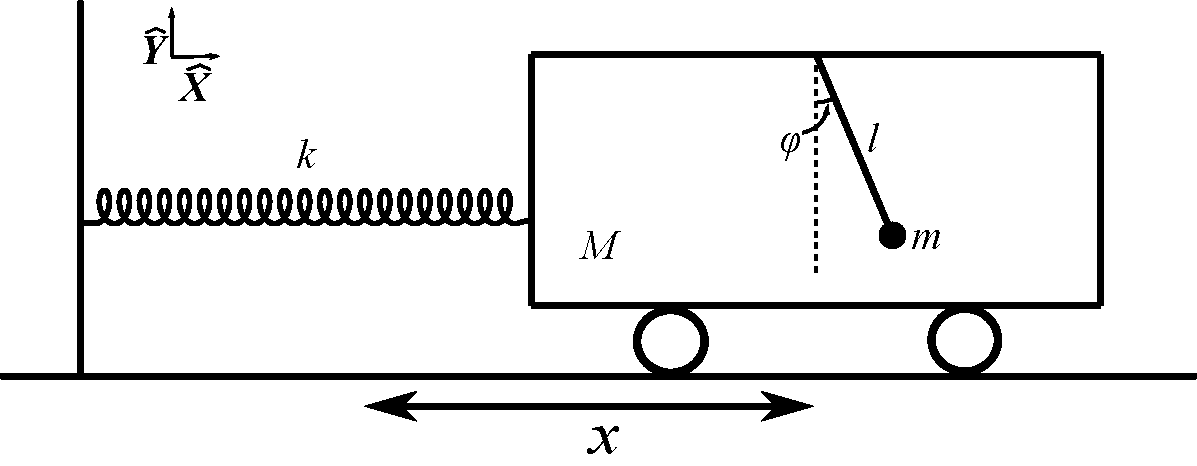
\includegraphics[width=.6\columnwidth]{Mekanik/mekfigs/PendulIVogn.pdf}
\caption{Illustration af situationen med indtegnet kartesisk koordinatsystem og genereliserede koordinater.}
\label{mek:fig:PendulIVogn}
\end{figure}
%
%
\begin{opgave}[4]{Pendul i en vogn}
\opg Origo defineres som ophængningspunktet for pendulet for $X=0$, og koordinatsystemet placeres således at tyngdekraften er i $Y$-retningen og fjederkraften er i $X$-retningen, se \cref{mek:fig:PendulIVogn}.
%
\opg De kartesiske koordinater for pendullodets position er
%
\begin{align*}
	X_p &= x + l\sin\phi, \\
	Y_p &= l\cos\phi.
\end{align*}
%
og for vognet er $Y_v$ uændret, da den kun kan bevæge sig langs $\hat{X}$, hvorfor den er ubetydelig. Slutteligt er
%
\begin{align*}
	X_v = x.
\end{align*}
%
\opg Vognens forskydning er den eneste, som betyder noget for fjederen, og pendullodets vertikale position bruges til den gravitationelle den, hvorved
%
\begin{align*}
	V = \frac{1}{2}kx^2 + mgl(1-\cos\phi).
\end{align*}
%
\opg Differentieres de kartesiske koordinater fås
\begin{align*}
	\dot{x}_p &= \dot{x} + l\dot{\phi}\cos\phi, \\
	\dot{y}_p &= l\dot{\phi}\sin\phi, \\
	\dot{x}_v &= \dot{x}.
\end{align*}
%
Det ses at idiotformlen kan anvendes ved kvadrering, analogt til \cref{k-mek:eq:SmartFart} i kompendiet, hvorved der opnås
%
\begin{align*}
	K = \frac{1}{2}M\dot{x} + \frac{1}{2}m\big[\dot{x}^2 + l^2\dot{\phi}^2 + 2l\dot{x}\dot{\phi}\cos\phi\big].
\end{align*}
%
hvorfor Lagrangefunktionen bliver
%
\begin{align*}
	L = \frac{1}{2}M\dot{x} + \frac{1}{2}m\big[\dot{x}^2 + l^2\dot{\phi}^2 + 2l\dot{x}\dot{\phi}\cos\phi\big] - \frac{1}{2}kx^2 + mgl(1-\cos\phi).
\end{align*}
%
\opg Differentialerne  for $x$ bestemmes
%
\begin{align*}
	\pdv{L}{\dot{x}} &= M\dot{x}+ m\dot{x} + ml\dot{\phi}\cos\phi, \\
	\pdv{L}{x} &= -kx,\\
	\el{x} &= M\ddot{x}+ m\ddot{x} + ml(\ddot{\phi}\cos\phi - \dot{\phi}^2\sin\phi),
\end{align*}
%
hvilket giver differentialligningen
%
\begin{align*}
	a) \qquad M\ddot{x} + m\ddot{x} + ml\ddot{\phi}\cos\phi - ml\dot{\phi}^2\sin\phi &= -kx.
\end{align*}
%
Differentialerne for $\phi$ bestemmes
%
\begin{align*}
	\pdv{L}{\dot{\phi}} &= ml^2\dot{\phi} + ml\dot{x}\cos\phi, \\
	\pdv{L}{\phi} &= -ml\dot{x}\dot{\phi}\sin\phi - mgl\sin\phi,\\
	\el{\phi} &= ml^2\ddot{\phi} - ml\dot{x}\dot{\phi}\sin\phi + ml\ddot{x}\cos\phi,
\end{align*}
%
så differentialligningen bliver
%
\begin{align*}
	b) \qquad ml^2\ddot{\phi} + ml\ddot{x}\cos\phi &= -mgl\sin\phi.
\end{align*}
%
\opg Til første orden er $\cos\phi \simeq 1$, mens $\sin\phi \simeq \phi$ hvorved
%
\begin{align*}
    &a) \quad M\ddot{x} + m\ddot{x} +ml\ddot{\phi} \simeq -kx \\
    &b) \quad \ddot{\phi} + \frac{\ddot{x}}{l} \simeq -\frac{g}{l}\phi
\end{align*}
%
\opg Den svarer til følgende scenarier \\
%
1. \quad $k \implies \infty$ betyder at modstanden i fjederen bliver uendelig stor. \\
2. \quad Vognen er meget tungere end pendulet, som med andre ord betyder at vognen bevæger som om pendulet ikke var der.
%
\opg I de optalte grænser reducerer systemet til følgende situationer \\
%
1. \quad Modstanden i fjederen er så stor at vognen bevægelse bliver negligibel, hvorfor det forventes at pendulet opfører sig på sædvanlig vis, det vil sige en harmonisk oscillator\footnote{Den harmoniske oscillator kaldes også engang imellem simpel harmonisk bevægelse, forkortet SHB.}. \\
%
2. \quad Pendulets masse er så lille at dettes eksistens er ubetydelig for vognen, der så vil opføre sig som en vogn på en fjeder, altså en harmonisk oscillator. Det betyder for pendulet at dets ophængningspunkt vil oscillere harmonisk, hvorfor der forventes en drevet svingning af pendulet.
%
\opg Kigges på bevægelsesligningerne gøres følgende observationer \\
%
1. \quad Da $k$ er uendelig stor må $x$ være uendelig lille for at opfylde bevægelsesligningen og ligning $a$ mister herved betydning. Dette skal gælde til alle tider, så derfor må de tidsaflede af $x$ også være meget små, hvorfor de negligeres i $b$. Den eneste bevægelsesligning med betydning bliver derfor
%
\begin{align*}
	b) \quad \ddot{\phi} &= -\frac{g}{l}\phi = -\omega_1^2\phi \\
\phi &= A_1\cos(\omega_1t + \delta_1)
\end{align*}
%
hvor $A_1$ og $\delta_1$ begge er konstanter bestemt af startbetingelserne. \\
%
2. \quad Pendulets masse er negligibel ift. vognen, hvorfor led med $m$ negligeres fra bevægelsesligning $a$.
%
\begin{align*}
	a) \quad \ddot{x} &= -\frac{k}{M}x = -\omega_2^2x \\
	x &= A_2\cos(\omega_2t + \delta_2)
\end{align*}
%
hvor $A_2$ og $\delta_2$ igen er konstanter bestemt af startbetingelserne. Indsættes dette i bevægelsesligning $b$ fås
%
\begin{align*}
b) \quad \ddot{\phi} + \omega_1^2\phi = \frac{A\omega_2^2}{l}\cos(\omega_2t + \delta_2)
\end{align*}
%
hvor $\delta_2$ også er en konstant. Løsningen til denne differentialligning er træls, men det er en drevet harmonisk svingning. \\[2mm]
Konkluderende kan det siges at bevægelsesligningerne reducerer pænt til forventelige resultater i nogle udvalgte grænser, hvilket er en god indikator for deres validitet.
\end{opgave}


% \section*{Fiktive Kræfter}
% %
% %
% \begin{opgave}{Fysiske og fiktive kræfter}{2}
% \opg Det antages at systemet er stedafhængigt, hvilket vil sige at der udelukkende indgår variable i sted, hvilket eksempelvis kunne være de kartesiske koordinater $(x,y)$, og konstanter i den potentielle energi. $V(x,y)$ er dermed konstant overfor hastigheder $(\dot{x},\dot{y})$, hvorfor de partielt afledede mht. disse er $0$.
% \opg Af spørgsmål 1 er det led den potentielle energi bidrager til ledet $\el{\dot{q}_i}$ med $0$, hvis tidsafledede også er nul. Dermed er $\dif{t}{}\left(\pdif{\dd{t}{q}_i}{V}\right)=0$, hvilket giver den efterspurgte konklusion.
% \opg Eftersom den potentielle energi kun bidrager med et additivt led til delen af Euler \hspace{-0.1cm}- \hspace{-0.1cm}Lagrangeligningen, der er den generaliserede kraft, tilføjes differentialerne med negativt fortegn på den side af lighedstegnet, grundet  på Lagrangefunktionen.
% \opg Venstre side af lighedstegnene er masse gange acceleration, og summen af fysiske kræfter kan udtrykkes som den negative gradient af den samlede potentielle energi. Det betyder at hvis de fiktive kræfter betragtes som kræfter, så er ligningerne fra Newtons 2. lov i to forskellige dimensioner. Defineres de fiktive kræfter som i eksemplet opfører de sig dermed overfor Newtons 2. lov som enhver anden fysisk kraft.
% \end{opgave}
% %
% %
% \begin{figure*}
% 	\centering
% 	\includegraphics[width=.9\textwidth]{Analytisk-Mekanik/ToMasserRoterendeStangFiktivekrafter.pdf}
% 	\caption{De fiktive kræfter er her indtegnet hvor $m$, $\Omega$ og $\dd{t}{\rho}_1$ er antaget positive.} \label{mek:fig:ToMasserRoterendeStangFiktivekraefter}
% \end{figure*}
% %
% %
% \begin{opgave}{To masser på en roterende stang}{3}
% \opg Systemet roterer i et plan omkring et fast punkt, hvorfor cylindrisk polære koordinater er oplagt.
% \opg Da stangen er antaget stiv, kan loddernes bevægelse i $\phi$-retningen kun komme fra stangens rotation, som er antaget konstant. Da $\rho_1$ og $\rho_2$ er koblede er det generaliserede koordinat derfor enten $\rho_1$ eller $\rho_2$, og her vælges $\rho_1$.
% \opg Da stangens længde er konstant er
% \begin{align*}
% 	0 = \dif{t}{l}& = \dd{t}{\rho}_1 + \dd{t}{\rho}_2 \\
% 	\dd{t}{\rho}_1 &= -\dd{t}{\rho}_2
% \end{align*}
% \opg \cref{k-mek:eq:FiktiveKraefter} i kompendiet siger at\footnote{cor/cf står som superscript og ikke subscript for at gøre det mere overskueligt. Der er ikke anden grund.}
% \begin{align*}
% 	\va{F}^\textup{cor} &= 2m\dd{t}{\va{r}}\times\va{\Omega}, \\
% 	\va{F}^\textup{cf} &= m(\va{\Omega} \times \va{r}) \times \va{\Omega}.
% \end{align*}
% hvor de generaliserede koordinater på vektorform er
% \begin{align*}
% 	\va{\rho}_1 &= \rho_1\rhat, \\
% 	\va{\rho}_2 &= \rho_2\rhat = (l-\rho_1)\rhat,\\
% 	\dd{t}{\va{\rho}}_1 &= \dd{t}{\rho}_1\rhat, \\
% 	\dd{t}{\va{\rho}}_2 &= \dd{t}{\rho}_2\rhat = -\dd{t}{\rho}_1\rhat.
% \end{align*}
% Stangen roterer omkring $z$-aksen, hvorfor $\va{\Omega} = \Omega\zhat$. Derfor bliver de fiktive kræfter
% \begin{align*}
% 	\va{F}_1^\textup{cor} &= 2m_1\dd{t}{\rho}_1\Omega\rhat\times \zhat \\
% 	&= -2m_1\dd{t}{\rho}_1\Omega\phhat, \\
% 	\va{F}_1^\textup{cf}	&= m_1\rho_1\Omega^2(\zhat \times \rhat) \times \zhat \\
% 	&= m_1\rho_1\Omega^2(\phhat \times \zhat) \\
% 	&= m_1\rho_1\Omega^2\rhat, \\
% 	\va{F}_2^\textup{cor} &= 2m_2(-\dd{t}{\rho}_2)\Omega\rhat\times \zhat \\
% 	&= 2m_2\dd{t}{\rho}_2\Omega\phhat \\
% 	&= -2m_2\dd{t}{\rho}_1\Omega\phhat, \\
% 	\va{F}_2^\textup{cf} &= m_2\rho_2\Omega^2(\zhat \times \rhat) \times \zhat \\
% 	&= m_2\rho_2\Omega^2(\phhat \times \zhat) \\
% 	&= m_2\rho_2\Omega^2\rhat \\
% 	&= m_2(l-\rho_1)\Omega^2\rhat.
% \end{align*}
% \opg Antages $m$, $\Omega$ og $\dd{t}{\rho}_1$ for at være positive fås \cref{mek:fig:ToMasserRoterendeStangFiktivekraefter}.
% \opg Corioliskraften virker på begge legemer i $\phhat$-retningen, men stangen er antaget stiv, hvorfor den påvirker legemerne med en ligestor og modsatrettet normalkraft, hvilket er samme argument som for at $\phi$ ikke er et generaliseret koordinat.
% \opg I systemets ligevægtskonfiguration er de to centrifugalkræfters vektorsum nul
% \begin{align*}
% 	\va{F}_1^\textup{cf} + \va{F}_2^\textup{cf} &= \va{0} \\
% 	\implies m_1\rho_1\Omega^2 &= m_2\rho_2\Omega^2 \\
% 	\implies \frac{m_1}{m_2} &= \frac{\rho_2}{\rho_1} = \frac{l}{\rho_1} - 1.
% \end{align*}
% Vektoren $\rhat$ peger i hver sin retning for de to masser, hvorfor fortegnene passer. Af tegningen fremgår det at de er modsatrettet, og deres størrelser skal så være ens, hvilket er benyttet her.
% \opg Hvis masserne er ens forventes legemerne at placere sig lige langt fra rotationspunktet, dvs. $\rho_1 = \rho_2$.
% \opg Indsættes de forventede omstændigheder fås
% \begin{align*}
% 	\frac{m_1}{m_1} = \frac{\rho_1}{\rho_1} \quad \checkmark
% \end{align*}
% \end{opgave}
% %
% %
% \begin{opgave}{Er fiktive kræfter trælse?}{3}
% \opg Corioliskraften afhænger af hastighed, mens centrifugalskaften afhænger af position.
% \opg Typisk er kræfter stedafhængige, hvilket gælder f.eks. gravitation, fjederkræfter og elektriske kræfter. Derfor giver centrifugalkraften "bare"\;en ekstra stedafhængighed, hvilket ikke er helt umuligt, mens hastighedsafhængigheden af Corioliskraften gør den bøvlet at arbejde med.
% \opg Denne differentialligning minder ret så meget om
% \begin{align*}
% 	\dif{t}{g(t)} = kg(t)
% \end{align*}
% Den minder faktisk så meget om, at de er ens hvis $g(t) = \dif{t}{f(t)}$
% \begin{align*}
% 	\dif{t}{}\left(\dif{t}{f(t)}\right) = k\left(\dif{t}{f(t)}\right),
% \end{align*}
% hvorfor løsningen af denne differentialligningen kan bruges
% \begin{align*}
% 	\dif{t}{f(t)} = g(t) = A\exp(kt),
% \end{align*}
% hvor separation af de variable kan benyttes
% \begin{align*}
% 	\d f &= A\exp(kt)\dd{t} \\
% 	\int \d f &= \int A\exp(kt)\dd{t} \\
% 	f(t) &= \frac{A}{k}\exp(kt) + B.
% \end{align*}
% Her er konstanterne fra begge ubestemte integraler lagt ind i konstanten $B$.
% \end{opgave}
% %
% %
% \section*{Perspektiverende Problemer}
% %
% %
% \begin{opgave}{Tennis Racket Theorem}{4}
% Det vigtige her er først at forstå antagelsen om de små vinkelaccelerationer. Eksempelvis er $\omega_y$ ikke lille nok til at se bort fra alle led, der indeholder $\omega_y$, men den er lille nok til at $\omega_y^2 \approx 0$, hvorfor alle led der indeholder $\omega_y^2$, $\omega_z^2$ eller $\omega_y\omega_z$ kan negligeres.
% \opg Derved er
% \begin{align*}
% 	\dif{t}{}\left(I_x\dd{t}{\omega}_x\right) \simeq \dif{t}{}\left[(I_y-I_z)(0)\right] = 0.
% \end{align*}
% Generelt set er
% \begin{align*}
% 	\dif{t}{}(\omega_i\omega_j) = \dd{t}{\omega}_i\omega_j + \omega_i\dd{t}{\omega}_j.
% \end{align*}
% Vi har dog lige argumenteret for at $\dd{t}{\omega}_x \simeq 0$, hvilket betyder led, der afhænger af $\dd{t}{\omega}_x$ negligeres. Herved opnås \cref{mek:eq:TRT_DiffLignX} ved at differentiere den anden vinkelhastighed.
% \opg I \cref{mek:eq:TRT_DiffLign} isoleres de relevante førsteafledede og så indsættes det i \cref{mek:eq:TRT_DiffLignX}.
% \opg Eftersom $I_x>I_y$ er $I_x-I_y > 0$, mens $I_z<I_x$, hvorfor $I_z-I_x<0$. Vinkelhastighederne er reelle, hvorfor
% \begin{align*}
% 	\omega_x^2(I_z-I_x)(I_x-I_y) < 0.
% \end{align*}
% Idet inertimomenterne er positive størrelser, ændres fortegnet ikke at at dividere med $I_y$ eller $I_z$, hvilket betyder at $\ddt{\omega}_i \propto -\omega_i$ for $i=y,z$, hvilket er den ønskede konklusion.
% \opg I første omgang differentieres, hvor det huskes at andenordensled i $\omega_x$ og $\omega_z$ negligeres
% \begin{align*}
% 	\dif{t}{}\xyz{I_x\dd{t}{\omega}_x}{I_y\dd{t}{\omega}_y}{I_z\dd{t}{\omega}_z} = \xyz{(I_y-I_z)\omega_y\dd{t}{\omega}_z}{0}{(I_x-I_y)\dd{t}{\omega}_x\omega_y}.
% \end{align*}
% Bruges \cref{mek:eq:TRT_DiffLign} her til at substituere i de enkeltafledede fås \cref{mek:eq:TRT_DiffLignY}.
% \opg Analogt til spørgsmål 3) fås at $(I_y-I_z)$ og $(I_x-I_y)$ er positive, hvorfor
% \begin{align*}
% 	\omega_y^2(I_x-I_y)(I_y-I_z) > 0,
% \end{align*}
% hvor fortegnet igen ikke ændres af at dividere med $I_x$ eller $I_z$.
% \opg Hvis rotationen skal være stabil, så må legemet ikke bevæge sig ret meget omkring de andre akser. Har $\ddt{\omega}_j$ samme fortegn som $\omega_j$ så vil vinkelhastigheden øges eksponentielt i tiden, hvorfor legemets rotation om den $j$'te akse øges kraftigt, hvis den ikke starter med en startvinkelhastighed $\omega_j = 0$. Dette betyder at legemets rotation vil starte en rotation om de sekundære\footnote{Den primære rotationsakse er den akse med ikke-lille startværdi af vinkelhastigheden, mens de sekundære akser er dem, hvor startrotationen er lille.} akser, hvorfor rotationen er ustabil. Har $\omega_j$ og $\ddt{\omega}_j$ modsat fortegn så vil vinkelhastighed oscillere omkring 0. Det betyder at legemets rotation får vinklen ved de sekundære akser til at holde sig omkring deres startværdi grunden antagelsen om små vinkelhastigheder.
% \opg Fra spørgsmål 3) og spørgsmål 5) samt opgaveteksten til spørgsmål 7 har vi at rotationen om de sekundære akser accelereres, hvis $y$-aksen er den primære rotationsakse, mens der induceres en oscillation omkring de sekundære akser, hvis $x$ eller $z$ er den primære akser. Derved er $y$-aksen ustabil, mens de andre to er stabile.
% \opg For en kasse, bog eller andet rektangulært objekt er det således
% %
% %
% \begin{figure}[!h]
% \centering
% 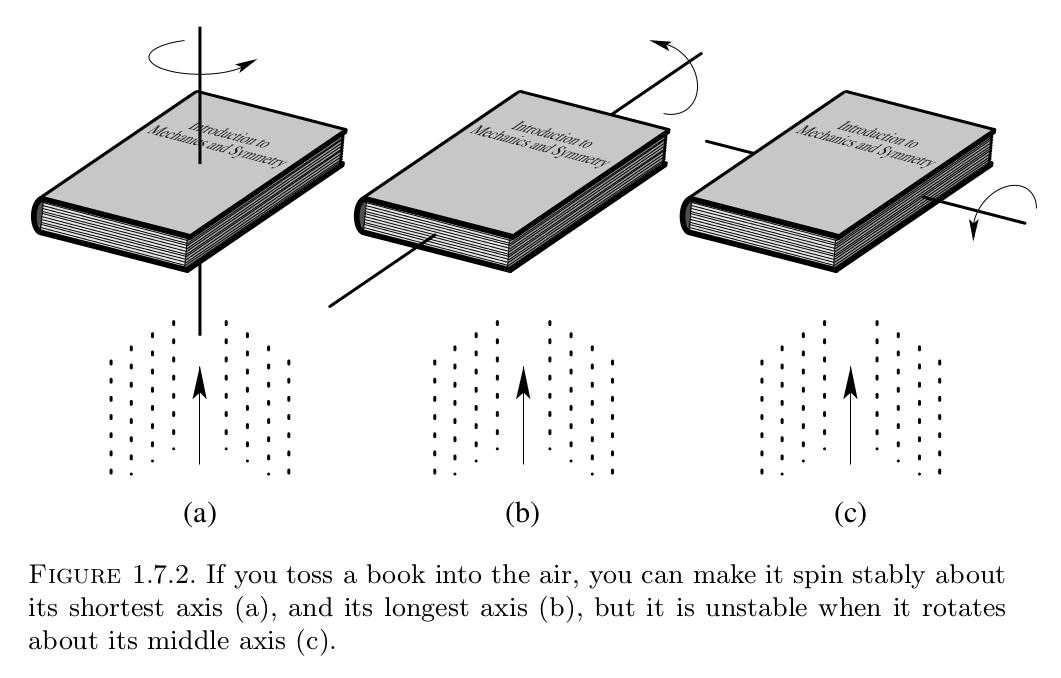
\includegraphics[width=.85\columnwidth]{Analytisk-Mekanik/Rotationsakser.png}
% \caption{Illustration af en bog, der roterer med forskellige primærakser, samt en beskrivelse af deres stabilitet.}
% %\caption{Kilde: \newline \url{https://physics.stackexchange.com/questions/67957/stability-of-rotation-of-a-rectangular-prism0}}
% \end{figure}
% \end{opgave}
% %
% %
% \begin{opgave}{Hamiltonfunktionen og et systems energi}{3}
% \opg $L = \frac{1}{2}A(q)\dd{t}{q}^2 - V(q)$.
% \opg $p = \pdif{\dd{t}{q}}{L} = A(q)\dd{t}{q}$.
% \opg $\dd{t}{q} = \frac{p}{A(q)}$.
% \opg $H = p\dd{t}{q} - L = \frac{p^2}{A(q)} - \left( \frac{p^2}{2A(q)} - V(q)\right) = \frac{p^2}{2A(q)} + V(q)$.
% \opg Der er to måder at vise dette på. Den mest stringente er at starte med energien, udtrykt ved sted og impuls er
% \begin{align*}
% 	E = K + V = \frac{1}{2}A(q)\dd{t}{q}^2 + V(q) = \frac{p^2}{2A(q)} + V(q) = H.
% \end{align*}
% Den anden metode er følgende: Pr. antagelse er $K = \frac{1}{2}A(q)\dd{t}{q}^2$. Dette omskrives nu ved den generaliserede impuls fra spørgsmål 3)
% \begin{align*}
% 	K &= \frac{1}{2}A(q)\dd{t}{q}^2 \\
% 	&= \frac{1}{2}A(q)\left(\frac{p}{A(q)}\right)^2 \\
% 	&= \frac{p^2}{2A(q)}.
% \end{align*}
% Indsættes det i Hamiltonfunktionen fra spørgsmål 4) fås definitionen på total energi
% \begin{align*}
% 	H &= \frac{p^2}{2A(q)} + V(q) = K + V = E.
% \end{align*}
% \opg Taleargumentet lyder på at ingen af disse argumenter bygger på andet end antagelsen om formen af energierne. Derfor ændres intet når der tilføjes flere koordinater og der summeres. \\
% Et mere matematisk argument er at den kinetiske energi nu skrives på formen
% \begin{align*}
% 	K = \sum_i\frac{1}{2}A(q_i)\dd{t}{q}_i^2,
% \end{align*}
% mens den potentielle energi er $V(q_1,q_2,...,q_n)$. Derfor er Lagrangefunktionen
% \begin{align*}
% 	L = \sum_i\frac{1}{2}A(q_i)\dd{t}{q}_i^2 -  V(q_1,q_2,...,q_n).
% \end{align*}
% Benyttes definitionen af generaliseret impuls, samt det faktum at der ingen krydsled er i den del af Lagrangefunktionen, der afhænger af $\dd{t}{q
% }_i$, fås at
% \begin{align*}
% 	q_i = \frac{p_i}{A(q_i)}.
% \end{align*}
% Den kinetiske energi kan nu skrives på formen
% \begin{align*}
% 	K = \sum_i\frac{p_i^2}{2A(q_i)},
% \end{align*}
% og sættes disse to ligninger ind i definitionen på Hamiltonfunktionen fås
% \begin{align*}
% 	H &= \sum_ip_iq_i - L \\
% 	&= \sum_ip_i\frac{p_i}{A(q_i)} - \left(\sum_i\frac{p_i^2}{2A(q_i)} -  V(q_1,q_2,...,q_n)\right) \\
% 	&= \frac{p_i^2}{2A(q_i)} +  V(q_1,q_2,...,q_n) \\
% 	&= K + V = E.
% \end{align*}
% Som bonusinformation kan det siges, at selvom Hamiltonfunktionen har den omtalte form, så er det ikke nødvendigvis den mest logiske måde at definere systemets energi på. I nogle tilfælde giver det mere mening at definere energien anderledes, hvilket er muligt, da det absolutte energi ikke har den store betydning i sig selv, da det er ændringer i energien, som har betydning for systemets opførsel. Dette benyttes eksempelvis i \cref{k-mek:sec:PendulLagrange} i kompendiet om beskrivelsen af pendulet i Lagrangeformalismen, hvor den potentielle energi defineres til at være $0$ i pendulets ligevægtspunkt.
% \end{opgave}
% %
% %
% \begin{opgave}{Fra klassisk mekanik til kvantemekanik}{3}
% Kvantemekanikken bygger på Hamiltonformalismen, hvorfor idéen med denne opgave er at introducere Hamiltonfunktionen, der omskrives til Hamiltonoperatoren, $\op{H}$, som kan betragtes som grundstenen for kvantemekanikken, fordi den tidsuafhængige eller stationære Schrödingerligning kan skrives som egenværdiproblemet
% \begin{align}
% 	\op{H}\psi = E\psi.
% \end{align}
% Her går $\psi$'erne ikke ud med hinanden, da dette er formuleret ved hjælp af den gren af matematikken, der hedder lineær algebra, hvilket gør matematikken meget lettere, når først man har styr på denne matematik\footnote{Der er lidt fyldtekst fra tid til anden idet dette oprindelig var skrevet som en del af kompendiet, og det bliver beholdt, da det ikke er dårlig indformation, selvom det dog ikke er nødvendigt for at løse opgave.}. Hamiltonoperatoren kan opskrives ud fra den klassiske Hamiltonfunktion.
% \opg Den generaliserede impuls kan skrives på formen $p = m\dd{t}{q}$, hvorfor $\dd{t}{q} = p/m$. Derved bliver den kinetiske energi
% \begin{align} \label{mek:eq:K(p)}
% 	K = \frac{1}{2}m\dd{t}{q}^2 = \frac{1}{2}m\left(\frac{p}{m}\right)^2 = \frac{p^2}{2m}.
% \end{align}
% \opg Derved giver \cref{k-mek:eq:H=E} i kompendiet at
% \begin{align}
% 	H = K + V = \frac{p^2}{2m} + V.
% \end{align}
% \opg Sted og impuls skal omskrives til operatorer, mens masse er en partikelegenskab, og ikke en observabel, med tilhørende operator.
% \opg Benyttes impulsoperatoren fra \cref{k-mek:tab:operatorer_i_kvant} i kompendiet nu, samt definitionen på tallet $i$, nemlig at $i^2 = -1$ fås Hamiltonoperatoren fra samme tabel
% \begin{align}
% 	\op{x} &= x \implies \op{V} = V \\
% 	\op{p}^2 &= \left(-i\hbar\pdif{x}{}\right)^2 = -\hbar^2\pdif[2]{x}{} \\
% 	\implies \op{H} &= \frac{\op{p}^2}{2m} + \op{V} = -\frac{\hbar^2}{2m}\pdif[2]{x}{} + V
% \end{align}
% Der er hermed dannet en bro mellem klassisk mekanik og kvantemekanik, og målet med dette er at vise at en sådan bro eksisterer fremfor en rigid gennemgang af Hamiltonformalismen og dens klassiske mangfoldigheder. \\

% Konkluderende kan det siges at metoden til at analysere et kvantemekanisk system er at opskrive systemets kinetiske\footnote{Der er stort set aldrig krydsled i den kinetiske energi, hvorfor dette ofte er trivielt.} og potentielle energi, for derefter at opstille systemets Hamiltonfunktion. Denne omskrives til en Hamiltonoperator, som giver mening for systemet, og derefter løses den staionære Schrödingerligning. Dette kan lyde relativt simpelt, men der kan komme en del komplikationer i forbindelse med eksempelvis skridtet med at omskrive Hamiltonfunktionen til en passende Hamiltonoperator.
% \end{opgave}
% %
% %
% \begin{opgave}{Energibevarelse i Hamilton}{4}
% \opg Ved partiel differentiation, f.eks. $\partial/\partial t$, betragtes alt andet end den variabel der differentieres med hensyn til som konstanter og der tages dermed ikke højde for at nogle variable kan afhænge af den variabel, der differentieres med hensyn til. Den fuldstændige tidsaflede tager højde for eventuelle implicitte afhængigheder og kædereglen benyttes til at udtrykke disse. Som eksempel kan bruges et generaliseret koordinat $q$
% \begin{align*}
% 	\pdif{t}{q} &= 0, \\
% 	\dif{t}{q} &= \dd{t}{q},
% \end{align*}
% og det illustreres endnu tydeligere ved $q^2$
% \begin{align*}
% 	\pdif{t}{q^2} &= 0,\\
% 	\dif{t}{q^2} &= \pdif{q}{q^2}\dif{t}{q} = (2q)\dd{t}{q} = 2q\dd{t}{q}.
% \end{align*}
% \opg Kædereglen benyttes til at skrive den fuldstændigt tidsafledede af en generel Hamiltonfunktion
% \begin{align} \label{mek:eq:dHdt}
% 	\dif{t}{}H(q,p,t) = \pdif{q}{H}\dif{t}{q} + \pdif{p}{H}\dif{t}{p} + \pdif{t}{H}.
% \end{align}
% Dette gøres da en generel éndimensionel Hamiltonfunktion afhænger eksplicit af tid, det generaliserede koordinat og den dertilhørende generaliserede impuls, og med den fuldstændige tidsafledede skal der tages højde for at de to sidstnævnte kan være tidsafhængige.
% \opg Hamiltonsligninger siger
% \begin{align*}
% 	\pdif{q}{H} &=  -\dd{t}{p}, \\
% 	\pdif{p}{H} &=  \dd{t}{q}.
% \end{align*}
% Indsættes det i \cref{mek:eq:dHdt} fås
% \begin{align*}
% 	\dif{t}{H} &= -\dd{t}{p}\dif{t}{q} + \dd{t}{q}\dif{t}{p} + \pdif{t}{H}, \\
% 	\dif{t}{H} &= -\dd{t}{p}\dd{t}{q} + \dd{t}{q}\dd{t}{p} + \pdif{t}{H}.
% \end{align*}
% \opg Dette følger trivielt fra ovenstående spørgsmål
% \begin{align*}
% 	\dif{t}{H} = \pdif{t}{H}.
% \end{align*}
% \opg Hamiltonfunktionen er bevaret i tid, hvis den ikke ændrer sig i tid, hvilket skrives matematisk som $\d H/\dd{t} = 0$, og det er opfyldt hvis $H$ ikke er eksplicit tidsafhængig, altså $\partial H/\partial t = 0$. Da Lagrangefunktionen og Hamiltonfunktionen har samme eksplicitte tidsafhæninghed medfører dette at Hamiltonfunktionen også er bevaret i tid, hvis $\partial L/\partial t = 0$. Dermed er systemets energi bevaret, hvis systemet opfylder at Hamiltonfunktionen er systemets energi og at denne ikke er eksplicit tidsafhængig.
% \opg Dette gøres ved at tilføje $i$'er på $q$ og $p$ og summe over disse led
% \begin{align*}
% 	\dif{t}{H} = \sum_i\left[\pdif{q_i}{H}\dif{t}{q_i} + \pdif{p_i}{H}\dif{t}{p_i}\right] + \pdif{t}{H}.
% \end{align*}
% Præcis samme fremgangsmåde benyttes da ingen af argumenterne er specifikke på en sådan måde så de ikke gælder for et arbitrært koordinat.
% \begin{align*}
% 	\dif{t}{H} &= \sum_i\bigg[-\dd{t}{p}\dd{t}{q} + \dd{t}{q}\dd{t}{p}\bigg] + \pdif{t}{H} = \pdif{t}{H},
% \end{align*}
% da indholdet af parentesen er nul for alle $i$
% \begin{align*}
% 	-\dd{t}{p}\dd{t}{q} + \dd{t}{q}\dd{t}{p} = 0 \enspace \forall \; i.
% \end{align*}
% Konklusionen er derfor den samme: Hvis Hamilton-/Lagrangefunktionen ikke er eksplicit tidsafhængig, så er systemets energi bevaret.
% \end{opgave}


\end{document}